\documentclass{beamer}

\mode<presentation>
{
  \usetheme[compress]{Berlin}
  \usecolortheme{default}
  %\usefonttheme{serif}
  %\usepackage{fontspec}
  %\setmainfont{Liberation Serif}
  %\usetheme{default}      % or try Darmstadt, Madrid, Warsaw, ...
  %\usecolortheme{default} % or try albatross, beaver, crane, ...
  \usefonttheme{default}  % or try serif, structurebold, ...
  \setbeamertemplate{navigation symbols}{}
  \setbeamertemplate{caption}[numbered]
} 
\addtobeamertemplate{navigation symbols}{}{%
    \usebeamerfont{footline}%
    \usebeamercolor[fg]{footline}%
    \hspace{1em}%
    \insertframenumber/\inserttotalframenumber
}
\usepackage{multicol}
\usepackage[utf8]{inputenc}
\usepackage[T1]{fontenc}
\usepackage[english]{babel}
\usepackage{parskip}
\usepackage{array}
\usepackage{xspace}
\usepackage{amsmath}
\usepackage{amssymb}
\usepackage{amsthm}
\usepackage{nccmath}
\usepackage{biblatex}
\graphicspath{ {./figures/} }
\usepackage{longtable}
\usepackage[dvipsnames]{xcolor}
\usepackage{graphicx} 
\usepackage{xmpmulti}
\usepackage{booktabs} 
\let\lemma\relax
\newtheorem{lemma}[theorem]{\gr Λήμμα}
\newtheorem{mycorollary}[theorem]{Corollary}
\newtheorem{myprop}[theorem]{Proposition}
\theoremstyle{definition}
\newcommand{\en}{\selectlanguage{english}}
\newcommand{\gr}{\selectlanguage{greek}}
\newcommand{\A}{\mathcal{A}}
\newcommand{\STRUCT}{\text{STRUCT}}


\title[]{Graph attention networks and expressiveness}
\author[Georgiadou, Pappas]{Ilektra Styliani Georgiadou, Thomas Pappas}
\institute[ALMA]{}
\date{\today}

\begin{document}
\AtBeginSection[]{
  \begin{frame}
  \vfill
  \centering
  \begin{beamercolorbox}[sep=8pt,center,shadow=true,rounded=true]{title}
    \usebeamerfont{title}\insertsectionhead\par%
  \end{beamercolorbox}
  \vfill
  \end{frame}
}


\begin{frame}[plain]
  \titlepage
  \begin{columns}
\column{0.4\textwidth}
    \begin{figure}
      \centering
      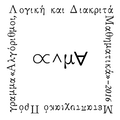
\includegraphics[scale=0.6]{alma_logo.png}
    \end{figure}
\column{0.5\textwidth}
ALMA \\
\tiny{INTER-INSTITUTIONAL GRADUATE PROGRAM \\
"ALGORITHMS, LOGIC AND DISCRETE MATHEMATICS"}
\end{columns}
\end{frame}

\begin{frame}
    \frametitle{Table of Contents}
    \tableofcontents[hideallsubsections]
\end{frame}


\section{Graph Attention Networks}

\begin{frame}{Past GNN approaches}
    Past GNN attempts include spectral and non-spectral approaches
    \begin{itemize}
        \item Spectral: Compute and depend on the Laplacian eigenvalues
            \begin{itemize}
                \item computation is demanding, though it has been improved over time
                \item dependant on the graph structure
            \end{itemize}
        \item Non-spectral: define convolutions directly on the graph
            \begin{itemize}
                \item dependent on the neighborhood size (learn for each node degree)
                \item or learn on a fixed neighborhood size (GraphSAGE)
            \end{itemize}
    \end{itemize}
\end{frame}

\begin{frame}{Graph Convolutional Neural Networks}
    \textbf{GCN} is a type of convolutional neural network that can work directly on graphs and take advantage of their structural information.\\
    \bigskip \pause
    \begin{block}{In General}
        For each node, we get the feature information from all its neighbors and itself. We will use the same function for all the nodes. Finally, we feed the result values into a neural network. We can also stack more layers on top of each other to get a deeper GCN. The output of a layer will be treated as the input for the next layer.
    \end{block} \pause
    The way GCN aggregates messages is structure-dependent, which may hurt its generalizability.
\end{frame}

\begin{frame}{Graph Attention Networks}
    GAT introduces the attention mechanism as a substitute for the statically normalized convolution operation.
    \begin{block}{Attention Strategy}
        Compute the hidden representations of each node in the graph, by attending over its neighbours, following a self-attention strategy, which will be: 
        \begin{enumerate}
            \item Efficient (parallelizable)
            \item Applied to nodes of different degrees
            \item Applicable to inductive learning problems
        \end{enumerate}
    \end{block} \pause
    Given as input a set of node features \(h=\{\vec{\rm h_{1}},\dots,\vec{\rm h_{N}}\},\;\vec{\rm h_{i}}\in \mathbb{R}^{F}\), produce a new set of node features \(h'=\{\vec{\rm h'_{1}},\dots,\vec{\rm h'_{N}}\},\;\vec{\rm h'_{i}}\in \mathbb{R}^{F'}\)
\end{frame}

\begin{frame}{Graph Attentional Layer}
    \begin{block}{Single layer Algorithm}
    \textbf{Input:} set of node features \(h=\{\vec{\rm h_{1}},\dots,\vec{\rm h_{N}}\}\), weight matrix \(W\in \mathbb{R}^{F'\times F}\) (learnable), shared attentional mechanism \(\alpha: \mathbb{R}^{F'}\times\mathbb{R}^{F'}\rightarrow \mathbb{R}\), nonlinearity function \(\sigma\)
    \begin{itemize}
        \item Compute attention coefficients for nodes \(j\in \mathcal{N}_{i}\) as \(e_{ij}=\alpha(\textbf{W}\vec{\rm h_{i}},\textbf{W}\vec{\rm h_{j}})\), the importance of node \(j\)'s features to \(i\)
            \begin{itemize}
                \item Can be done across all nodes or only within the neighborhood (masked attention)
            \end{itemize}
        \item Normalize them as \(\alpha_{ij}=softmax_{j}(e_{ij})=\frac{exp(e_{ij})}{\sum_{k\in\mathcal{N}_{i}}exp(e_{ik})}\)
        \item Compute linear combination and (potentially) apply a nonlinearity \(\sigma\), \(\vec{\rm h'_{i}}=\sigma\left(\sum_{j\in\mathcal{N}_{i}}\alpha_{ij}\textbf{W}\vec{\rm h_{j}}\right)\)
    \end{itemize}
    \end{block}
    
\end{frame}


\begin{frame}{Multi-head attention}
    To stabilize the learning process, we employ multi-head attention, so we execute the last step of the Algorithm for \(K\) independent attention mechanisms and their features are concatenated.\\
    \bigskip \pause
    Performing multi-head attention on the final layer, taking averages and nonlinearity function \(\sigma\), so:
    \[\vec{\rm h'_{i}}=\sigma\left(\frac{1}{K}\sum_{k=1}^{K}\sum_{j\in\mathcal{N}_{i}}\alpha_{ij}^k\textbf{W}^k\vec{\rm h_{j}}\right)\]
\end{frame}

\begin{frame}{Illustrations}
    \begin{multicols}{2}
        \begin{figure}
            \centering
            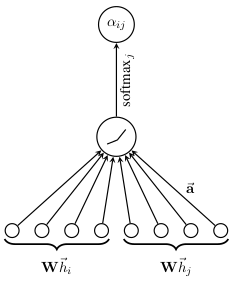
\includegraphics[scale=0.4]{GAT1.png}
            \caption{The attention mechanism \(\alpha(\textbf{W}\vec{\rm h_{i}},\textbf{W}\vec{\rm h_{j}})\) parametrized by a weight vector \(\vec{\rm a}\)}
        \end{figure}
        \begin{figure}
            \centering
            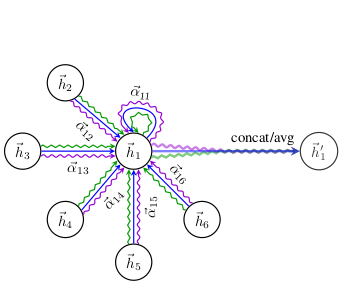
\includegraphics[scale=0.40]{GAT2.png}
            \caption{Multi-head attention where different arrow colors denote independent attention computations}
        \end{figure}
    \end{multicols}
\end{frame}

\begin{frame}{Effectiveness}
    Parallelization of computations
    \begin{itemize}
        \item Self-attentional layer // across all edges
        \item Output features // across all nodes
    \end{itemize} \pause
    \begin{block}{Time Complexity}
        Time needed in a single GAT attention head computing \(F'\) features and \(F\) input features for graph \(G(V,E)\) is:
        \begin{center}
            \(\mathcal{O}(\;|V|FF'+|E|F'\;)\)
        \end{center}
    \end{block} \pause
    Applying multi-head attention multiplies the storage and parameter requirements by a factor of \(K\). The individual heads’ computations are fully independent.
\end{frame}

\begin{frame}{Benefits}
    \begin{itemize}
        \item Allows assigning different importances to nodes of the same neighborhood
        \item Analyzing the learned attentional weights may lead to benefits in interpretability (e.g. in the machine translation domain)
        \item Applied in a shared manner to all edges in the graph, without upfront access to the global graph structure, so:
        \begin{itemize}
            \item there is no need for undirected graphs
            \item it is directly applicable to inductive learning
        \end{itemize}
        \item Works with the entirety of the neighborhood and does not assume any ordering within it
        \begin{itemize}
            \item Opposite to previous inductive methods with fixed-sized neighborhoods and the existence of a sequential node ordering across neighborhoods (GraphSAGE)
        \end{itemize}
    \end{itemize}
\end{frame}

\begin{frame}{Evaluation}
    In all experiments
    \begin{itemize}
        \item Masked attention has been applied on first-order neighbors
        \item The attention mechanism \(\alpha\) is a single-layer  feedforward  neural  network
            \begin{itemize}
                \item parametrized by a weight vector \(\vec{\rm{a}}\in \mathbb{R}^{2F^\prime}\)
                \item LeakyReLU nonlinearity (with negative input slope \(\alpha = 0.2\)) is applied
            \end{itemize}
    \end{itemize}
\end{frame}

\begin{frame}{Test: Transductive learning}
    \begin{block}{Dataset}
        Three standard  citation  network  benchmark  datasets were utilised: Cora, Citeseer and Pubmed. Nodes correspond to documents and edges to (undirected) citations.  Node features correspond to elements of a bag-of-words representation of a document.
    \end{block} \pause
    \begin{block}{Methods}
        Comparison is done against the approaches specified in Kipf \& Welling (2017).
        \begin{itemize}
            \item Same metrics were used
            \item Maximum performance is reported
            \item Also included GCN-64, a GCN model that computes 64 hidden features using ReLU or ELU activation
        \end{itemize}
    \end{block}
\end{frame}

\begin{frame}{Test: Transductive learning}
    \begin{block}{Setup}
        Two-layer GAT model
        \begin{itemize}
            \item First layer
                \begin{itemize}
                    \item \(K=8\) attention heads
                    \item \(F^\prime = 8\) features each
                    \item ELU nonlinearity
                \end{itemize}
            \item Second layer: Classification
                \begin{itemize}
                    \item Single attention head (\(8\) for Pubmed)
                    \item \(C\) features (number of classes)
                    \item Softmax activation
                \end{itemize}
        \end{itemize}
        Due to low number of training nodes (\(140, 120, 60\) respectively)\\
        \(L_2\) regularisation is applied with \(\lambda = 0.0005\) (\(0.001\) for Pubmed) and dropout \(p = 0.6\) to all inputs and attention coefficients.
    \end{block}
\end{frame}

\begin{frame}{Test Results: Transductive learning}
    \begin{tiny}
    \begin{table}
      \caption{Transductive}
      \label{table:1}
      \begin{tabular}{ l l l l }
        \hline
        Method & Cora & Citeseer & Pubmed \\
        \hline
        MLP & $55.1\%$ & $46.5\%$ & $71.4\%$ \\
        ManiReg (Belkin et al., 2006) & $59.5\%$ & $60.1\%$ & $70.7\%$ \\
        SemiEmb (Weston et al., 2012) & $59.0\%$ & $59.6\%$ & $71.7\%$ \\
        LP (Zhu et al., 2003) & $68.0\%$ & $45.3\%$ & $63.0\%$ \\
        DeepWalk (Perozzi et al., 2014) & $67.2\%$ & $43.2\%$ & $65.3\%$ \\
        ICA (Lu \& Getoor, 2003) & $75.1\%$ & $69.1\%$ & $73.9\%$ \\
        Planetoid (Yang et al., 2016) & $75.7\%$ & $64.7\%$ & $77.2\%$ \\
        Chebyshev (Defferrard et al., 2016) & $81.2\%$ & $69.8\%$ & $74.4\%$ \\
        GCN (Kipf \& Welling, 2017) & $81.5\%$ & $70.3\%$ & $79.0\%$ \\
        MoNet (Monti et al., 2016) & $81.7\pm0.5\%$ & — & $78.8\pm0.3\%$ \\
        \hline
        GCN-64 & $81.4\pm0.5\%$ & $70.9\pm0.5\%$ & $79.0\pm0.3\%$ \\
        GAT (Velickovic et al., 2018) & $83.0\pm0.7\%$ & $72.5\pm0.7\%$ & $79.0\pm0.3\%$ \\
        \hline
      \end{tabular}
    \end{table}
    \end{tiny}
\end{frame}

\begin{frame}{Test: Inductive learning}
    \begin{block}{Dataset}
        A protein-protein interaction (PPI) dataset was utilised. Dataset consists of graphs corresponding to different human tissues.
    \end{block}
    \begin{block}{Methods}
        Comparison is done against four different super-vised GraphSAGE inductive methods presented in Hamilton et al. (2017).
    \end{block} \pause
    \begin{block}{Const-GAT}
        A variation Const-GAT is also provided with a constant attention mechanism \(\alpha(x,y) = 1\). This will assign the same weight to every neighbor and can be used to strictly evaluate the benefits of applying an attention mechanism (i.e. comparing with a near GCN-equivalent model).
    \end{block}
\end{frame}

\begin{frame}{Test: Inductive learning}
    \begin{block}{Setup}
        Three-layer GAT model
        \begin{itemize}
            \item First and Second layer
                \begin{itemize}
                    \item \(K = 4\) attention heads
                    \item \(F^\prime = 256\) features each
                    \item ELU nonlinearity
                \end{itemize}
            \item Third layer: Multi-label classification
                \begin{itemize}
                    \item \(K = 6\) attention heads
                    \item \(F^\prime = 121\) features each
                    \item Avaraged followed by Sigmoid activation
                \end{itemize}
        \end{itemize}
        No regularisation or dropout is required\\
        (\(44906\) training nodes from \(20\) graphs).
    \end{block}
\end{frame}

\begin{frame}{Test Results: Inductive learning}
    \begin{small}
    \begin{table}
      \caption{Inductive}
      \label{table:2}
      \begin{tabular}{ l l }
        \hline
        Method & PPI \\
        \hline
        Random & $0.396$ \\
        MLP & $0.422$ \\
        GraphSAGE-GCN (Hamilton et al., 2017) & $0.500$ \\
        GraphSAGE-mean (Hamilton et al., 2017) & $0.598$ \\
        GraphSAGE-LSTM (Hamilton et al., 2017) & $0.612$ \\
        GraphSAGE-pool (Hamilton et al., 2017) & $0.600$ \\
        \hline
        GraphSAGE & $0.768$ \\
        Const-GAT (Velickovic et al., 2018) & $0.934\pm0.006$ \\
        GAT (Velickovic et al., 2018) & $0.973\pm0.002$ \\
        \hline
      \end{tabular}
    \end{table}
    \end{small}
\end{frame}


\section{How Powerful are GNNs?}
\begin{frame}{Representational Power of GNNs}
    \begin{block}{Background}
    GNNs are widely used and have state-of-the-art results, but there is a lack of a theoretical framework to analyse their expressive power and what graph structures they can capture.
    \end{block} \pause
    \begin{block}{Key insight}
    Use the GNNs' similarities to the Weisfeiler-Lehman Isomorphism Test to evaluate their ability to distinguish graphs.
    \end{block}
\end{frame}

\begin{frame}{Background}
    \begin{block}{Multiset}
    A set that allows multiple instances.\\
    Formally $X$ is a multiset when $X = (S, m)$ where
    \begin{itemize}
        \item $S$ is the set of the distinct elements of $X$
        \item $m: S \rightarrow \mathbb{N}_{\geq1}$ the multiplicity of the elements
    \end{itemize}
    \end{block}
\end{frame}

\begin{frame}{Weisfeiler-Lehman Isomorphism Test}
    Test to evaluate weather two graphs are isomorphic.
    \begin{block}{Algorithm}
    For two Graphs $G_1, G_2$, for each node
    \begin{enumerate}
        \item Assign an initial label (same for all nodes)
        \item Create a multiset of the labels of all its neighbouring nodes
        \item Create a hash using its label and multiset and update its label with it 
        \item Repeat steps 2 - 3 until the labels' values stop changing
    \end{enumerate}
    If at any step the labels of the nodes between $G_1,G_2$ differ then they are not isomorphic.
    \end{block}
    A positive answer works well for most graphs.
\end{frame}

\begin{frame}
    \transduration<0-7>{0}
    \multiinclude[<+->][format=png, graphics={width=\textwidth}]{WL}
\end{frame}


\begin{frame}{Theoretical Framework}
    \begin{block}{Intuition}
    A maximally powerful GNN should map two nodes with different neighborhood structure to different locations. Therefore its aggregation scheme needs to be injective.
    \end{block}
\end{frame}

\begin{frame}{Conditions for Powerful GNNs (1/2)}
    \begin{block}{Lemma 2 (Xu et al. (2019))}
    Let \(G_{1}\) and \(G_{2}\) be any two non-isomorphic graphs. If a graph neural network \(\A : \mathcal{G} \rightarrow \mathbb{R}^d\) maps \(G_{1}\) and \(G_{2}\) to different embeddings, the Weisfeiler-Lehman graph isomorphism test also decides \(G_{1}\) and \(G_{2}\) are not isomorphic.
    \end{block}
\end{frame}

\begin{frame}{Conditions for Powerful GNNs (2/2)}
    \begin{block}{Theorem 3 (Xu et al. (2019))}
    Let \(\A: G \rightarrow \mathbb{R}^d\) be a GNN. With a sufficient number of GNN layers, \(\A\) maps any graphs \(G_1\) and \(G_2\) that the Weisfeiler-Lehman test of isomorphism decides as non-isomorphic, to different embeddings if the following conditions hold:
    \begin{enumerate}
        \item \(\A\) aggregates and updates node features iteratively with
            \[
                h_v^{(k)} = \phi\left(h_v^{(k-1)},f\left(\Big\{h_u^{(k-1)}:u\in \mathcal{N}(v)\Big\}\right)\right)
            \]
            where the functions \(f\), which operates on multisets, and \(\phi\) are injective.
        \item \(\A\)’s graph-level readout, which operates on the multiset of node features \(\Big\{h_v^{(k)}\Big\}\), is injective.
    \end{enumerate}
    \end{block}
\end{frame}

\begin{frame}{Graph Isomorphism Network}
    We will first see that sum aggregators can represent universal functions over multisets
    \begin{block}{Lemma 5 (Xu et al. (2019))}
    Assume \(\mathcal{X}\) is countable. There exists a function \(f:\mathcal{X} \rightarrow \mathbb{R}^n\) so that \(h(X) = \sum_{x\in X} f(x)\) is unique for each multiset \(X \subset \mathcal{X}\) of bounded size.  Moreover, any multiset function \(g\) can be decomposed as \(g(X) = \phi\left(\sum_{x\in X}f(x)\right)\) for some function \(\phi\).
    \end{block}
\end{frame}

\begin{frame}{Graph Isomorphism Network}
    \begin{footnotesize}
    The following aggregation scheme (among many other potential ones) will satisfy the condition \(1\) of the Theorem.
    \begin{block}{Corollary 6 (Xu et al. (2019))}
    Assume \(\mathcal{X}\) is countable.  There exists a function \(f:\mathcal{X} \rightarrow \mathbb{R}^n\) so that for infinitely many choices of \(\epsilon\), including all irrational numbers,
    \[
        h(c,X) = (1 + \epsilon) \cdot f(c) + \sum_{x\in X}f(x)
    \]
    is unique for each pair \((c,X)\), where \(c\in\mathcal{X}\) and \(X \subset \mathcal{X}\) is a multiset of bounded size. Moreover, any function \(\phi\) over such pairs can be decomposed as
    \[
        g(c,X) = \phi\left((1 + \epsilon) \cdot f(c) + \sum_{x\in X}f(x)\right)
    \]
    for some function \(\phi\). \(\epsilon\) can be either a learnable parameter or a fixed scalar.
    \end{block}
    \end{footnotesize}
\end{frame}

\begin{frame}{Graph Isomorphism Network}
    We can use multi-layer perceptrons (MLPs) to model and learn \(f\) and \(\phi\). Therefore GIN will update the node representations using
    \[
        h_v^{(k)} = MLP^{(k)}\left(\left(1+\epsilon^{(k)}\right) \cdot h_v^{(k-1)} + \sum_{u\in \mathcal{N}(v)}h_u^{(k-1)}\right)
    \]
    For graph classification, as features from earlier iterations may generalize better, we concatenate across all iterations/layers of GIN
    \[
        %h_G = CONCAT\left(READOUT\left(\Big\{h_v^{(k)}|v\in G\Big\}\right) | k = 0, 1, \dots , K\right)
        h_G = CONCAT\left(\sum_{v\in G}h_v^{(k)} \Big | k = 0, 1, \dots , K\right)
    \]
\end{frame}

\begin{frame}{Less Powerful GNNs}
    \begin{itemize}
        \item Mean aggregators (e.g. GCN)
            \begin{itemize}
                \item cannot distinguish some node structures, but captures the distribution
            \end{itemize}
        \item Max-pooling (e.g. GraphSAGE) or Min-pooling aggreagators
            \begin{itemize}
                \item even weaker, but can identify representative elements
                \item ignores multiplicities, i.e. reduces the multiset to a simple set
            \end{itemize}
    \end{itemize}
\end{frame}

\begin{frame}{Less Powerful GNNs}
    \begin{figure}
        \centering
        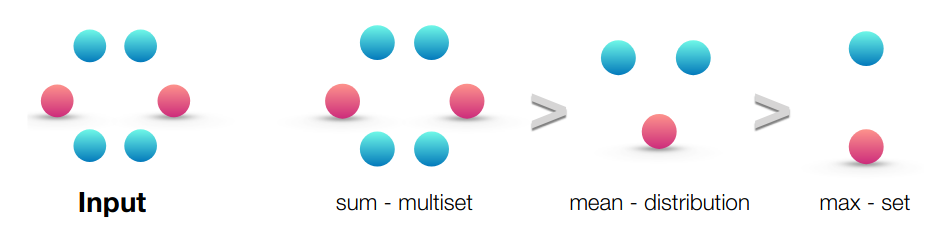
\includegraphics[scale=0.9]{expr_power_ranking.png}
        \caption{Ranking by expressive power for sum, mean and max aggregators over a multiset}
    \end{figure}
    \begin{figure}
        \centering
        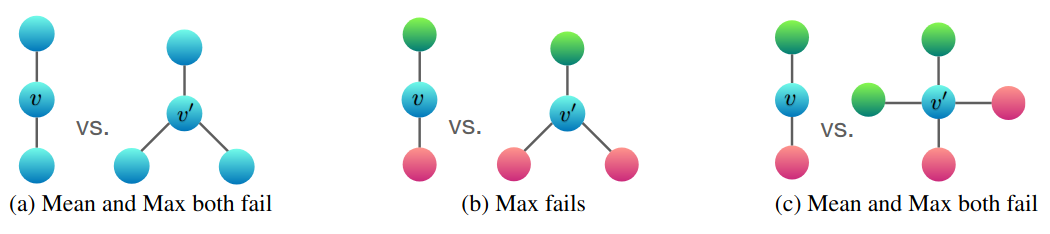
\includegraphics[scale=0.9]{struc_fail_distinguish.png}
        \caption{Examples of graph structures that mean and max aggregators fail to distinguish.}
    \end{figure}
\end{frame}

\begin{frame}{Experiments}
    \begin{block}{Datasets}
        We use 9 graph classification benchmarks
        \begin{itemize}
            \item 4 bioinformatics datasets (MUTAG, PTC, NCI1, PROTEINS)
            \item 5 social network datasets (COLLAB, IMDB-BINARY, IMDB-MULTI, REDDIT-BINARY, REDDIT-MULTI5K)
        \end{itemize}
        We want the models to learn from network structure, so we put no features.
    \end{block}
\end{frame}

\begin{frame}{Experiments}
    \begin{block}{Models}
        \begin{itemize}
            \item GIN-\(\epsilon\): a GIN that learns \(\epsilon\)
            \item GIN-\(0\): a GIN where \(\epsilon = 0\)
            \item GIN-\(0\) with a 1-layer perceptron
            \item MLP with a MEAN aggregator
            \item GCN
            \item MLP with a MAX aggregator
            \item GraphSAGE
        \end{itemize}
    \end{block}
\end{frame}

\begin{frame}{Experimens}
    \begin{block}{Configuration}
        A \(10\)-fold cross-validation is performed and the average and standard deviation of validation accuracies is reported.\\
        \bigskip
        For all models
        \begin{itemize}
            \item 5 GNN layers (including input)
            \item MLPs have \(2\) layers
            \item Batch normalisation is applied
        \end{itemize}
    \end{block}
    \begin{block}{Training accuracy}
        Training accuracy is also reported (5 GNN layers) along with the WL subtree kernel (4 iterations comparable to the 5 GNN layers).
    \end{block}
\end{frame}

\begin{frame}{Experiments}
    \begin{figure}
        \centering
        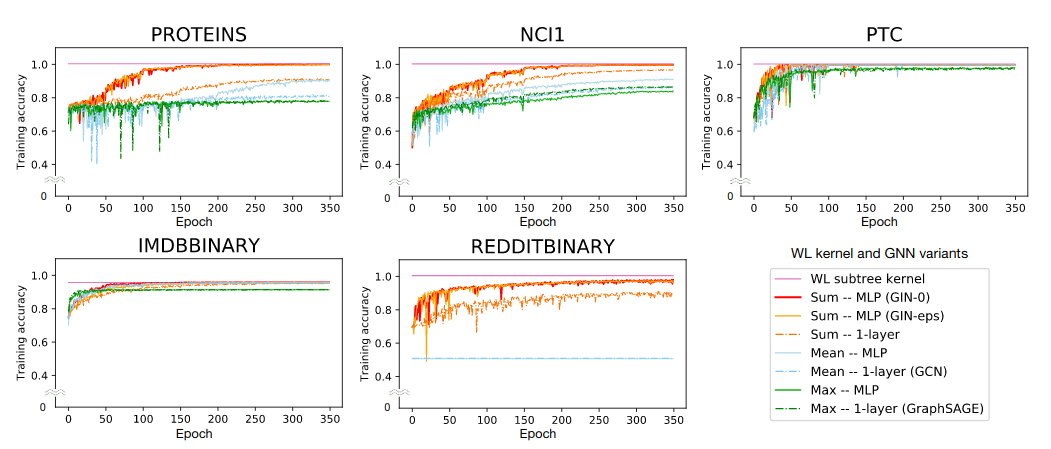
\includegraphics[scale=1]{gins_training_set_perf.png}
        \caption{Training set performance of GINs, less powerful GNN variants and the WL subtree kernel}
    \end{figure}
\end{frame}

\begin{frame}{Experiments}
    \begin{tiny}
    \begin{table}
      \caption{Test set classification accuracies (\%) (social networks)}
      \label{table:3}
      \begin{tabular}{ l c c c c c }
        \hline
        Datasets & IMDB-B & IMDB-M & RDT-B & RDT-M5K & COLLAB \\
        \hline
        SUM–MLP (GIN-\(0\)) & $75.1\pm5.1$ & $52.3\pm2.8$ & $92.4\pm2.5$ & $57.5\pm1.5$ & $80.2\pm1.9$ \\
        SUM–MLP (GIN-\(\epsilon\)) & $74.3\pm5.1$ & $52.1\pm3.6$ & $92.2\pm2.3$ & $57.0\pm1.7$ & $80.1\pm1.9$ \\
        SUM–1-LAYER7 & $4.1\pm5.0$ & $52.2\pm2.4$ & $90.0\pm2.7$ & $55.1\pm1.6$ & $80.6\pm1.9$ \\
        MEAN–MLP & $73.7\pm3.7$ & $52.3\pm3.1$ & $50.0\pm0.0$ & $20.0\pm0.0$ & $79.2\pm2.3$ \\
        MEAN–1-LAYER (GCN) & $74.0\pm3.4$ & $51.9\pm3.8$ & $50.0\pm0.0$ & $20.0\pm0.0$ & $79.0\pm1.8$ \\
        MAX–MLP & $73.2\pm5.8$ & $51.1\pm3.6$ & – & – & – \\
        MAX–1-LAYER (GraphSAGE) & $72.3\pm5.3$ & $50.9\pm2.2$ & – & – & – \\
        \hline
      \end{tabular}
    \end{table}
    
    \begin{table}
      \caption{Test set classification accuracies (\%) (bioinformatics)}
      \label{table:4}
      \begin{tabular}{ l c c c c }
        \hline
        Datasets & MUTAG & PROTEINS & PTC & NCI1 \\
        \hline
        SUM–MLP (GIN-\(0\)) & $89.4\pm5.6$ & $76.2\pm2.8$ & $64.6\pm7.0$ & $82.7\pm1.7$ \\
        SUM–MLP (GIN-\(\epsilon\)) & $89.0\pm6.0$ & $75.9\pm3.8$ & $63.7\pm8.2$ & $82.7\pm1.6$ \\
        SUM–1-LAYER7 & $90.0\pm8.8$ & $76.2\pm2.6$ & $63.1\pm5.7$ & $82.0\pm1.5$ \\
        MEAN–MLP & $83.5\pm6.3$ & $75.5\pm3.4$ & $66.6\pm6.9$ & $80.9\pm1.8$ \\
        MEAN–1-LAYER (GCN) & $85.6\pm5.8$ & $76.0\pm3.2$ & $64.2\pm4.3$ & $80.2\pm2.0$ \\
        MAX–MLP & $84.0\pm6.1$ & $76.0\pm3.2$ & $64.6\pm10.2$ & $77.8\pm1.3$ \\
        MAX–1-LAYER (GraphSAGE) & $85.1\pm7.6$ & $75.9\pm3.2$ & $63.9\pm7.7$ & $77.7\pm1.5$ \\
        \hline
      \end{tabular}
    \end{table}
    \end{tiny}
\end{frame}

\begin{frame}{Experiments}
    \begin{block}{Results}
        \begin{itemize}
            \item WL subtree kernel is an upper bound, as predicted
            \item GINs achieve much higher performance that the other GNN variants
                \begin{itemize}
                    \item Followed by sum aggregators and then mean and max, again as predicted
                \end{itemize}
            \item GIN-\(0\) performs better than GIN-\(\epsilon\)
                \begin{itemize}
                    \item Probably due to its simplicity
                \end{itemize}
        \end{itemize}
    \end{block}
\end{frame}

\section{GCNs Loss of Expressive Power}
\begin{frame}{Intuition}
    \begin{block}{Goal}
        Theoretical analysis of the graph NN expressive power, by analyzing their asymptotic behaviors as the layer size goes to infinity.
    \end{block} \pause
    \begin{block}{General Approach}
        Using dynamical systems we will specialize to the GCNs, making use of a generalization of next Theorem. 
    \end{block}\pause
    \begin{block}{Theorem}
        If a finite and discrete Markov process is irreducible and aperiodic, it exponentially converges to a unique equilibrium and the eigenvalues of its transition matrix determine the convergence rate.
    \end{block}    
\end{frame}

\begin{frame}{Dynamical System}
    Definition of the problem:
    \begin{itemize}
        \item Function \(f_{l}:\mathbb{R}^{N\times C}\rightarrow\mathbb{R}^{N\times C}\) as \(f_{l}(X)=MLP_{l}(PX)=\sigma(\cdots\sigma(\sigma(PX)W_{l1})W_{l2}\cdots W_{lH_{l}})\), \\ the \(l-\)th multi-layer perceptron common to all nodes. 
        \begin{itemize}
            \item \(\sigma:\mathbb{R}^{N\times C}\rightarrow\mathbb{R}^{N\times C}\) is a ReLU function, \(P\in\mathbb{R}^{N\times N}\) is a symmetric matrix and \(W_{lh}\in\mathbb{R}^{C\times C}\)
        \end{itemize}
        \item Dynamics \(X^{(l+1)}=f_{l}(X^{(l)})\), with some initial value \(X^{(0)}\)
    \end{itemize}
    \bigskip
    We are interested in the asymptotic behavior of \(X^{(l)}\) as \(l\rightarrow\infty\).
\end{frame}

\begin{frame}{Dynamical System Results}
    Let \(U\) be a \(M-\)dimensional subspace of \(\mathbb{R}^{N}\)
    \begin{block}{Assumptions}
        \begin{enumerate}
            \item \(U\) has an orthonormal basis \((e_{m})_{m\in[M]}\) that consists of non-negative vectors.
            \item \(U\) is invariant under \(P\) , so if \(u \in U\) , then \(Pu \in U\).
        \end{enumerate}    
    \end{block} \pause
    Defining the subspace \(\mathcal{M}\) of \(\mathbb{R}^{N\times C}\) by \[\mathcal{M}=U\otimes\mathbb{R}^C=\{\sum_{m=1}^{M}e_{m}\otimes w_{m}|w_{m}\in \mathbb{R}^C\},\]  for \(X\in \mathbb{R}^{N\times C}\) denote distance between \(X\) and \(M\) by \(d_{\mathcal{M}}(X) := inf\{\|X-Y\|_{F} |\; Y \in \mathcal{M}\}\), the maximum singular value of \(W_{lh}\) by \(s_{lh}\) and \(\lambda:=\max_{n\in[N-M]}{|\lambda_{n}|}\), \(\lambda_{i}\) the eigenvalues of \(P\). 
\end{frame}

\begin{frame}{Dynamical System Results}
    \begin{block}{Theorem 1}
        Under Assumptions \(1\) and \(2\), we have 
        \begin{center}
            \(d_{\mathcal{M}}(f_{l}(X)) \leq s_{l}\lambda d_{\mathcal{M}}(X)\) for any \(X\in \mathbb{R}^{N\times C}\)  
        \end{center}
    \end{block}
    \begin{block}{Corollary 1}
        \(\mathcal{M}\) is invariant under \(f_{l}\) for any \(l\in\mathbb{N}_{+}\) , that is, if \(X\in\mathcal{M}\), then we have \(f_{l}(X)\in\mathcal{M}\).
    \end{block}
    \begin{block}{Corollary 2}
        Let \(s := \text{sup}_{l\in\mathbb{N}_{+}} s_{l}\). We have \(d_{\mathcal{M}}(X^{(l)}) = \mathcal{O}((s\lambda)^l)\). In particular, if \(s\lambda<1\), then \(X_{l}\) exponentially approaches \(\mathcal{M}\) as \(l\rightarrow\infty\) for any initial value \(X^{(0)}\).
    \end{block}
\end{frame}


\begin{frame}{Applications to GCNs}
    Let \(G=(V,E),\;|V|=N\) be an undirected graph, \(A\) be the adjacency matrix and \(D\) be the degree matrix of \(G\).\\
    \bigskip
    We define the augmented normalized Laplacian of \(G\) by \(\Delta:=I_{N}-(D+I_{N})^{-\frac{1}{2}}(A+I_{N})(D+I_{N})^{-\frac{1}{2}}\) and \(P:=I_{N}-\Delta\).\\
    \bigskip \pause
    For weights \(W_{l}\in \mathbb{R}^{C\times C}\), we define a GCN associated with \(G\) by \(f = f_{L}\circ\cdots\circ f_{1}\) where \(f_{l}:\mathbb{R}^{N\times C}\rightarrow\mathbb{R}^{N\times C}\) is defined by \(f_{l}(X) := \sigma(PXW_{l})\). \\
    \bigskip
    We are interested in the asymptotic behavior of the output \(X^{(L)}\) of the GCN as \(L \rightarrow\infty\).
    
\end{frame}

\begin{frame}{Applications to GCNs}
    For node classification tasks, we can interpret next result as the “information loss” of GCNs in the limit of infinite layers.
    \begin{block}{Theorem 2}
        For any initial value \(X^{(0)}\), the output of \(l-\)th layer \(X^{(l)}\) satisfies \(d_{\mathcal{M}}(X^{(l)})\leq(s\lambda)^{l}d_{\mathcal{M}}(X^{(0)})\). In particular, \(d_{\mathcal{M}}(X^{(l)})\) exponentially converges to \(0\) when \(s\lambda < 1\).
    \end{block} \pause
    For any \(X \in \mathcal{M}\), if two nodes \(i,j\in V\) are in a same connected component and their degrees are identical, then, the column vectors of \(X\) that correspond to nodes \(i\) and \(j\) are identical. \\
    \bigskip
    We cannot distinguish these nodes using X, so \(\mathcal{M}\) only has information about connected components and node degrees.
\end{frame}

\begin{frame}{Further Results for GCNs}
    \begin{block}{Theorem 3}
        Consider a GCN on the Erdős-Rényi graph \(G_{N,p}\) such that \(\frac{\log{N}}{N p} = o(1)\) as a function of \(N\). For any \(\epsilon > 0\), if the supremum \(s\) of the maximum singular values of weights in the GCN satisfies \(s < s_{0} := \frac{1}{7}\sqrt{\frac{Np-p+1}{\log{(4N/\epsilon)}}}\), then, for sufficiently large \(N\) , the GCN satisfies the condition of Theorem 2 with probability at least \(1-\epsilon\).
    \end{block} \pause
    The upper bound \(s_{0}\rightarrow\infty\) as \(N \rightarrow\infty\), so if the graph is sufficiently large and not extremely sparse, most GCNs suffer from information loss. For the dependence on the edge probability \(p, s_{0}\) is an increasing function of \(p\). \\
    \bigskip
    Theorem 3 implies that graph NNs perform poorly on dense NNs.
\end{frame}


% \begin{frame}{Experiments}
    
% \end{frame}


% \section{}
% \begin{frame}{Conclusion?}
    
% \end{frame}


\begin{frame}{Bibliography}
    \begin{itemize}
        \item Graph Attention Networks, by Petar Veličković, Guillem Cucurull, Arantxa Casanova, Adriana Romero, Pietro Liò and Yoshua Bengio
        \item How Powerful are Graph Neural Networks, by Keyulu Xu, Weihua Hu, Jure Leskovec and Stefanie Jegelka
        \item Graph Neural Networks Exponentially Lose Expressive Power for Node Classification, by Kenta Oono, Taiji Suzuki
        \item David Bieber, The Weisfeiler-Lehman Isomorphism Test
    \end{itemize}
\end{frame}

\begin{frame}{}
\centering
    \huge Thank you!
\end{frame}
\end{document}

